\documentclass[tikz,border=6pt]{standalone}
\usepackage{tikz}
\begin{document}
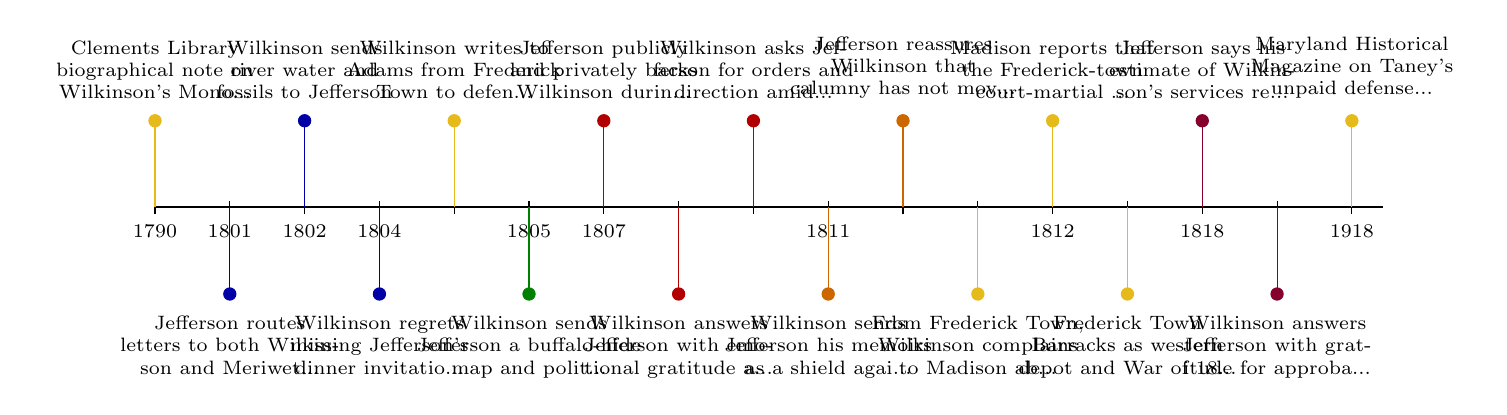
\begin{tikzpicture}[x=1cm,y=1cm]
\draw[thick] (0,0) -- (15.60,0);
\draw (0.00,0.08) -- (0.00,-0.08);
\node[font=\scriptsize, anchor=north] at (0.00,-0.10) {1790};
\draw (0.95,0.08) -- (0.95,-0.08);
\node[font=\scriptsize, anchor=north] at (0.95,-0.10) {1801};
\draw (1.90,0.08) -- (1.90,-0.08);
\node[font=\scriptsize, anchor=north] at (1.90,-0.10) {1802};
\draw (2.85,0.08) -- (2.85,-0.08);
\node[font=\scriptsize, anchor=north] at (2.85,-0.10) {1804};
\draw (3.80,0.08) -- (3.80,-0.08);
\draw (4.75,0.08) -- (4.75,-0.08);
\node[font=\scriptsize, anchor=north] at (4.75,-0.10) {1805};
\draw (5.70,0.08) -- (5.70,-0.08);
\node[font=\scriptsize, anchor=north] at (5.70,-0.10) {1807};
\draw (6.65,0.08) -- (6.65,-0.08);
\draw (7.60,0.08) -- (7.60,-0.08);
\draw (8.55,0.08) -- (8.55,-0.08);
\node[font=\scriptsize, anchor=north] at (8.55,-0.10) {1811};
\draw (9.50,0.08) -- (9.50,-0.08);
\draw (10.45,0.08) -- (10.45,-0.08);
\draw (11.40,0.08) -- (11.40,-0.08);
\node[font=\scriptsize, anchor=north] at (11.40,-0.10) {1812};
\draw (12.35,0.08) -- (12.35,-0.08);
\draw (13.30,0.08) -- (13.30,-0.08);
\node[font=\scriptsize, anchor=north] at (13.30,-0.10) {1818};
\draw (14.25,0.08) -- (14.25,-0.08);
\draw (15.20,0.08) -- (15.20,-0.08);
\node[font=\scriptsize, anchor=north] at (15.20,-0.10) {1918};
\filldraw[yellow!60!orange!90!black] (0.00,1.10) circle (2.2pt);
\draw[yellow!60!orange!90!black, thin] (0.00,0) -- (0.00,1.10);
\node[font=\scriptsize, align=center, text width=3.0cm, anchor=south] at (0.00,1.26) {Clements Library biographical note on Wilkinson's Mono...};
\filldraw[blue!65!black] (0.95,-1.10) circle (2.2pt);
\draw[blue!65!black, thin] (0.95,0) -- (0.95,-1.10);
\node[font=\scriptsize, align=center, text width=3.0cm, anchor=north] at (0.95,-1.26) {Jefferson routes letters to both Wilkinson and Meriwet...};
\filldraw[blue!65!black] (1.90,1.10) circle (2.2pt);
\draw[blue!65!black, thin] (1.90,0) -- (1.90,1.10);
\node[font=\scriptsize, align=center, text width=3.0cm, anchor=south] at (1.90,1.26) {Wilkinson sends river water and fossils to Jefferson};
\filldraw[blue!65!black] (2.85,-1.10) circle (2.2pt);
\draw[blue!65!black, thin] (2.85,0) -- (2.85,-1.10);
\node[font=\scriptsize, align=center, text width=3.0cm, anchor=north] at (2.85,-1.26) {Wilkinson regrets missing Jefferson's dinner invitatio...};
\filldraw[yellow!60!orange!90!black] (3.80,1.10) circle (2.2pt);
\draw[yellow!60!orange!90!black, thin] (3.80,0) -- (3.80,1.10);
\node[font=\scriptsize, align=center, text width=3.0cm, anchor=south] at (3.80,1.26) {Wilkinson writes to Adams from Frederick Town to defen...};
\filldraw[green!50!black] (4.75,-1.10) circle (2.2pt);
\draw[green!50!black, thin] (4.75,0) -- (4.75,-1.10);
\node[font=\scriptsize, align=center, text width=3.0cm, anchor=north] at (4.75,-1.26) {Wilkinson sends Jefferson a buffalo-hide map and polit...};
\filldraw[red!70!black] (5.70,1.10) circle (2.2pt);
\draw[red!70!black, thin] (5.70,0) -- (5.70,1.10);
\node[font=\scriptsize, align=center, text width=3.0cm, anchor=south] at (5.70,1.26) {Jefferson publicly and privately backs Wilkinson durin...};
\filldraw[red!70!black] (6.65,-1.10) circle (2.2pt);
\draw[red!70!black, thin] (6.65,0) -- (6.65,-1.10);
\node[font=\scriptsize, align=center, text width=3.0cm, anchor=north] at (6.65,-1.26) {Wilkinson answers Jefferson with emotional gratitude a...};
\filldraw[red!70!black] (7.60,1.10) circle (2.2pt);
\draw[red!70!black, thin] (7.60,0) -- (7.60,1.10);
\node[font=\scriptsize, align=center, text width=3.0cm, anchor=south] at (7.60,1.26) {Wilkinson asks Jefferson for orders and direction amid...};
\filldraw[orange!80!black] (8.55,-1.10) circle (2.2pt);
\draw[orange!80!black, thin] (8.55,0) -- (8.55,-1.10);
\node[font=\scriptsize, align=center, text width=3.0cm, anchor=north] at (8.55,-1.26) {Wilkinson sends Jefferson his memoirs as a shield agai...};
\filldraw[orange!80!black] (9.50,1.10) circle (2.2pt);
\draw[orange!80!black, thin] (9.50,0) -- (9.50,1.10);
\node[font=\scriptsize, align=center, text width=3.0cm, anchor=south] at (9.50,1.26) {Jefferson reassures Wilkinson that calumny has not mov...};
\filldraw[yellow!60!orange!90!black] (10.45,-1.10) circle (2.2pt);
\draw[yellow!60!orange!90!black, thin] (10.45,0) -- (10.45,-1.10);
\node[font=\scriptsize, align=center, text width=3.0cm, anchor=north] at (10.45,-1.26) {From Frederick Town, Wilkinson complains to Madison ab...};
\filldraw[yellow!60!orange!90!black] (11.40,1.10) circle (2.2pt);
\draw[yellow!60!orange!90!black, thin] (11.40,0) -- (11.40,1.10);
\node[font=\scriptsize, align=center, text width=3.0cm, anchor=south] at (11.40,1.26) {Madison reports that the Frederick-town court-martial ...};
\filldraw[yellow!60!orange!90!black] (12.35,-1.10) circle (2.2pt);
\draw[yellow!60!orange!90!black, thin] (12.35,0) -- (12.35,-1.10);
\node[font=\scriptsize, align=center, text width=3.0cm, anchor=north] at (12.35,-1.26) {Frederick Town Barracks as western depot and War of 18...};
\filldraw[purple!70!black] (13.30,1.10) circle (2.2pt);
\draw[purple!70!black, thin] (13.30,0) -- (13.30,1.10);
\node[font=\scriptsize, align=center, text width=3.0cm, anchor=south] at (13.30,1.26) {Jefferson says his estimate of Wilkinson's services re...};
\filldraw[purple!70!black] (14.25,-1.10) circle (2.2pt);
\draw[purple!70!black, thin] (14.25,0) -- (14.25,-1.10);
\node[font=\scriptsize, align=center, text width=3.0cm, anchor=north] at (14.25,-1.26) {Wilkinson answers Jefferson with gratitude for approba...};
\filldraw[yellow!60!orange!90!black] (15.20,1.10) circle (2.2pt);
\draw[yellow!60!orange!90!black, thin] (15.20,0) -- (15.20,1.10);
\node[font=\scriptsize, align=center, text width=3.0cm, anchor=south] at (15.20,1.26) {Maryland Historical Magazine on Taney's unpaid defense...};
\end{tikzpicture}
\end{document}
